\section{Initiating Interaction through Attention}
This section describes the design goals of our systems and their realization in particular interaction techniques.

\subsection{Design Goals}
Our work is motivated by the following design goals that leverage opportunities of head-worn computing, but also acknowledge potential challenges:

{\bf Leverage visual attention:} Take advantage of the fact that visual attention can express intention - initiate interaction based on where a user is already looking. 

{\bf Provide immediate feedback about selection targets in the environment:} While a near-eye display can push information to the user, users don't always want to control an object simply because they are looking at it (a problem known in gaze-based interaction as the Midas touch). A calmer~\cite{weiser_coming_1997} approach is to locate visual feedback about selection targets in the environment, to prevent distraction and interruption. Such feedback should be delivered instantaneously, while users look around a room.

{\bf Offer flexible orientation after initiating interaction:} After initiating attention through head orientation, enable the user to reorient their head or body position during the remaining interaction to prevent neck strain.

{\bf Offer efficient ways to disambiguate orientation input:} It may not always be possible to identify a unique target appliance based on a user's attention and orientation. Offer ways to supplement orientation-based interaction with screen-based interaction to provide disambiguation information.

These design goals find their expression in the following interaction model.

\subsection{Interaction Flow}

\begin{figure}[t!]
\centering
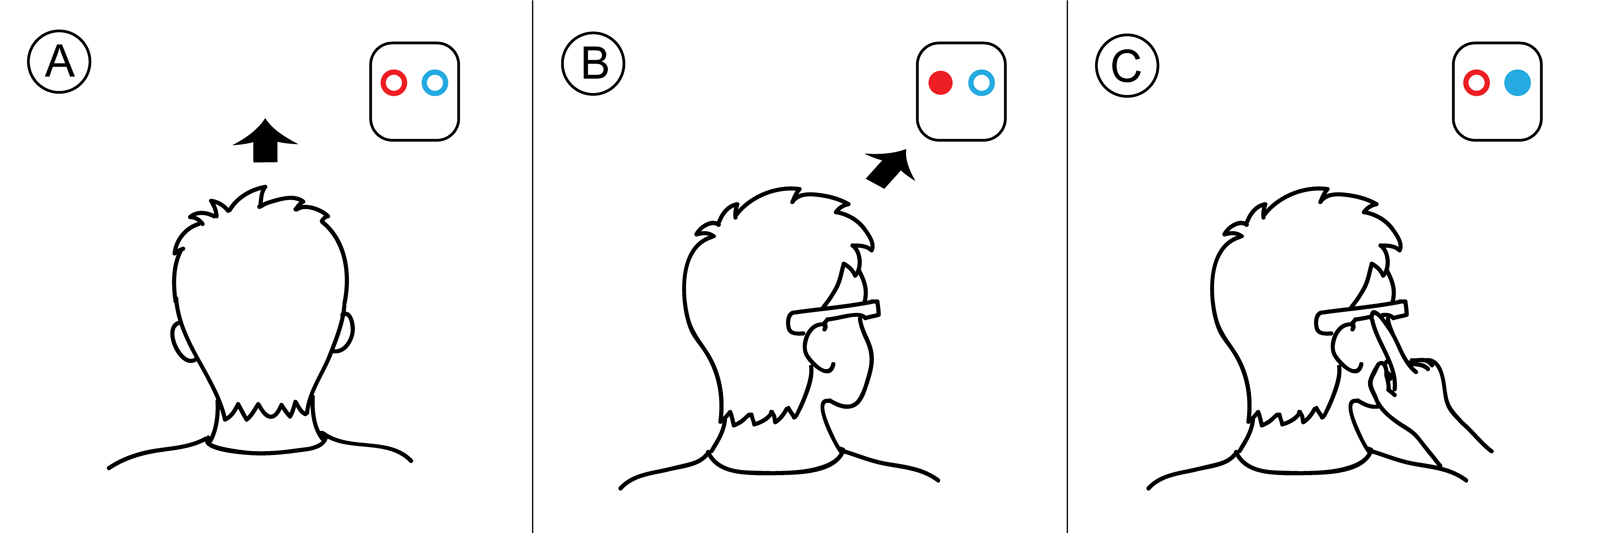
\includegraphics[width=\columnwidth]{figures/stepbystep_small.png}
\caption{Targeting interaction: when users turn towards a controllable appliance (A$\rightarrow$B), the appliance shows immediate visual feedback (red LED) (B). Users confirm that they wish to connect to this appliance with a tap (C) which triggers connection feedback (blue LED) on the appliance.}
\label{fig:interaction}
\end{figure}

\begin{figure}[t!]
\centering
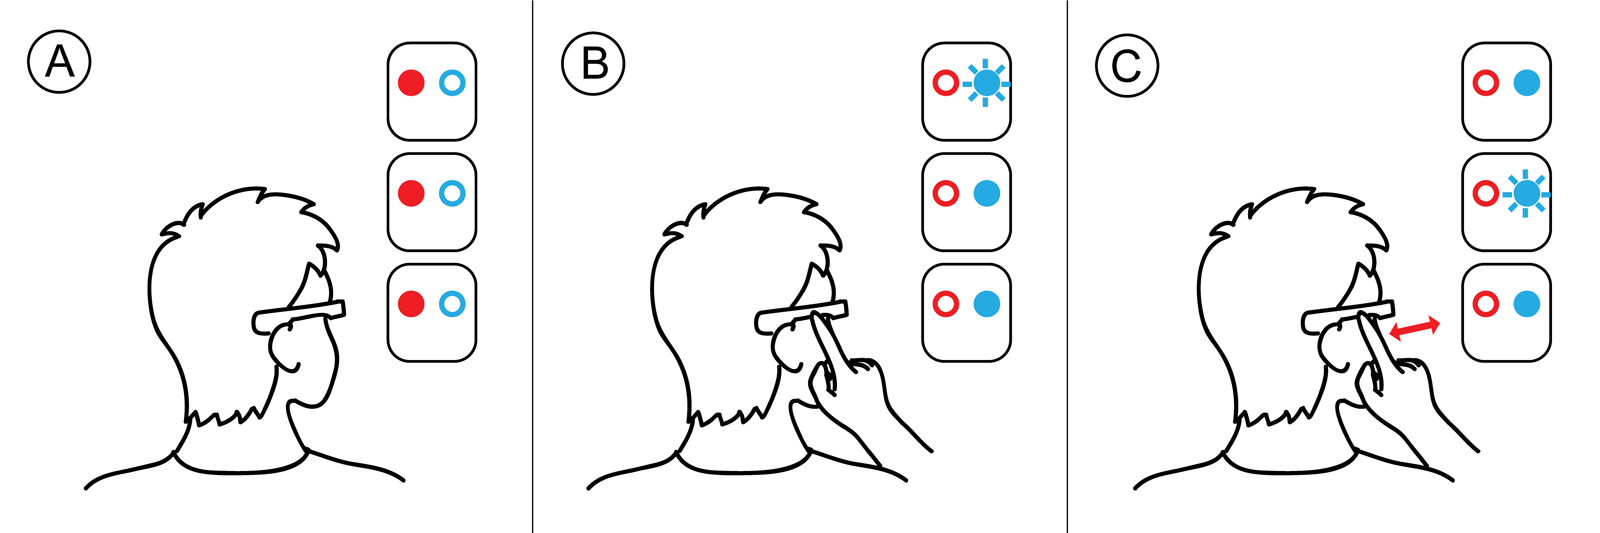
\includegraphics[width=\columnwidth]{figures/stepbystep_multi_small.png}
\caption{When multiple appliances are within range, they would all have red LEDs illuminated for feedback (A). Users call up the disambiguation where all responding clients lights up blue LED while the current hovered one blinks (B). Swiping on the touchpad to traverse among responding appliances (C).}
\label{fig:interaction_multi}
\end{figure}

{\bf Look:} Users select a target appliance by looking in its general direction.
Glass periodically sends a device id through its IR emitter analogous to Patel's approach~\cite{patel_2-way_2003}. Target appliances have IR receivers and offer immediate visual feedback by toggling a red LED whenever a valid id is received (Figure~\ref{fig:interaction}B). This enables {\em scanning} the environment with one's gaze to see which appliances can be controlled.

{\bf Initiate:} Users confirm their desire to connect to an appliance by tapping on the Glass touchpad. After connected, target appliance toggles on blue LED as visual feedback (Figure~\ref{fig:interaction}C). The next section on disambiguation deals with cases in which multiple appliances received valid IR signals. At this point, all further communication switches over to the 802.15.4 wireless network so that line of sight to the target is no longer needed.

{\bf Control:} Glass displays a user interface for parameters of the chosen appliance. Upon connected, the current status of the appliance is retreived by Glass and shown on the UI. The interface is controlled with the temple-mounted touchpad through the following gesture set: tapping toggles discrete parameters (such as power for a lamp as Figure~\ref{fig:ui_controls}(A)); single finger swipe changes between available parameters; double finger swipe adjusts continuous parameters (such as volume for a video player as Figure~\ref{fig:ui_controls}(B)). This scheme was chosen because the touchpad is only comfortably operable in the coronal plane (front to back) but not in the saggital plane (up and down). 
Control commands are sent over XBee radios.

{\bf Disengagement:} Users stay connected to the last selected appliance up to a timeout period. During that period, users can disengage through down swipes.

\begin{figure}[t!]
\centering
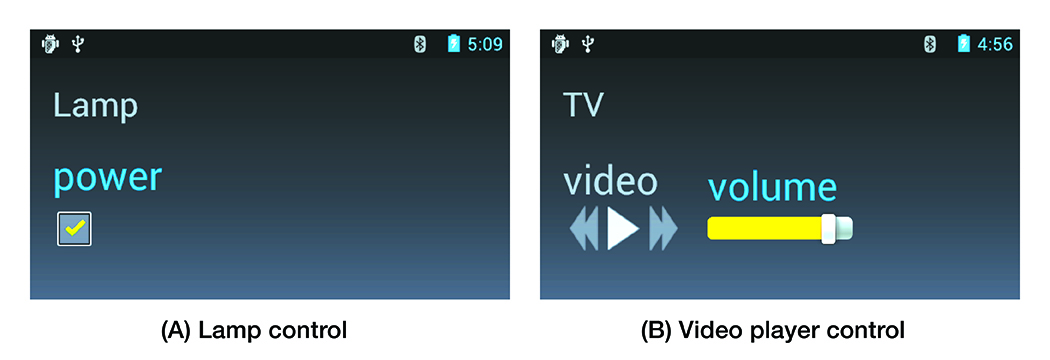
\includegraphics[width=\columnwidth]{figures/ui_controls_caption.jpg}
\caption{Screenshots of appliance controls}
\label{fig:ui_controls}
\end{figure}

\subsection{Disambiguation}
Head orientation only indicates a general area of visual interest. It does not necessarily match gaze orientation as extra-ocular muscles can move the eyes. The IR beam of our device also has a certain spread (see next section). In an environment dense with potential targets, multiple targets could be within range. Users can tell when multiple feedback LEDs in the environment illuminate (Figure~\ref{fig:interaction_multi}A). To disambiguate, users can either move to adjust their head position, or, alternatively, call up a disambiguation dialog on the Glass display. The dialog presents a list filtered to only those appliances that are within IR range, whlie appliances also use blue LED as visual cues: all responding appliances light up LEDs while the current hovered one blinks (Figure~\ref{fig:interaction_multi}B). Users navigate the list using the touchpad (Figure~\ref{fig:interaction_multi}C), and then continue their interaction as described above.
